% !TeX encoding = UTF-8
% !Tex program = Texmaker
% !Tex spellcheck = it_IT

\documentclass[binding=0.6cm,Lau]{sapthesis}

\usepackage{graphicx}
\usepackage{microtype}
\usepackage[italian]{babel}
\usepackage[utf8]{inputenc}
\usepackage{hyperref}
\hypersetup{pdftitle={La mia tesi},pdfauthor={Giacomo Colizzi Coin}}

\title{La mia tesi}
\author{Giacomo Colizzi Coin}
\IDnumber{1794538}
\course{Ingegneria informatica}
\courseorganizer{Facoltà di ingegneria dell'informazione, informatica e statistica}
\AcademicYear{2019/2020}
\copyyear{2020}
\advisor{Prof. Querzoni}
\authoremail{colizzicoin.1794538@studenti.uniroma1.it}

\begin{document}
\frontmatter
\maketitle

\begin{abstract}
Questa è la mia tesi
\end{abstract}

\tableofcontents

\mainmatter

\chapter{Introduzione}

Nella società attuale, programmare sta diventando sempre più comune e
alla portata di tutti.
% Inserire statistiche qui
Uno degli ambiti di interesse più comuni nella fascia di età citata è
quello dei videogiochi. Esistono molte piattaforme in cui un utente
può scegliere un gioco e giocarci liberamente, ed esistono anche
piattaforme che permettono di caricare i propri giochi. Queste
piattaforme richiedono però di avere dei requisiti particolari.
Inoltre, la velocità sempre crescente delle connessioni internet ha
permesso ai servizi di streaming di avere sempre più successo.

In questo contesto nasce l'idea di questa tesi.
Il progetto ha come obiettivo la creazione di una piattaforma per la
condivisione di videogiochi. Gli utenti di questa piattaforma possono
condividere con gli altri utenti i giochi da loro sviluppati. Tutti i
giochi caricati sulla piattaforma sono giocabili da ogni utente.
Infine, come utente, è possibile condividere le proprie esperienze di
gioco votando, commentando, invitando amici e altro.


\chapter{Requisiti, tecnologie e metodologie}

\section{Funzionalità offerte}

Come detto in precedenza, il sistema informativo progettato intende offrire agli utenti la possibilità di codividere, modificare e giocare ai videogiochi da loro sviluppati.
\newline
Chiunque voglia usufruire di questo servizio può creare un proprio account all'interno del sistema. I giochi caricati saranno visibili e giocabili da tutti gli altri utenti.
\newline
Per entrare nello scpecifico, passiamo ora alla descrizione delle funzionalità principali. Per comodità di esposizione, nella descrizione di queste divideremo l'analisi in sezioni e faremo riferimento diretto alle \textit{user stories}

\subsection{Sezione utenti}

Un visitatore del sito web che intende accedere al servizio deve ottenere le autorizzazione del sistema creando un account personale. Alla registrazione vengono richiesti un \textit{username}, un'\textit{email} valida e una \textit{password} per gli accessi futuri. In alternativa può registrarsi attraverso l'utilizzo della tecnologia \textit{OAuth}. Da questo momento in poi sarà definito \textit{giocatore}. Dopo aver confermato la sua registrazione, potrà accedere nuovamente al servizio fornendo le proprie credenziali. Avrà anche la possibilità di modificare le informazioni relative al proprio account.
\newline
Le user stories relative agli utenti sono le seguenti:
\textit{
\begin{enumerate}
\item Come visitatore, voglio creare un nuovo account, in modo che il sistema possa ricordarsi di me.
\item Come giocatore, voglio effettuare il login, in modo che possa interagire col sistema.
\item Come giocatore, voglio poter effettuare l'accesso con un account Google o Github.
\item Come giocatore, voglio poter terminare la sessione, così che il mio account sia protetto da usi non autorizzati.
\item Come giocatore, voglio poter modificare i dati del mio account, così che lo possa mantenere aggiornato.
\end{enumerate}
}

\begin{figure}[h!]
\centering
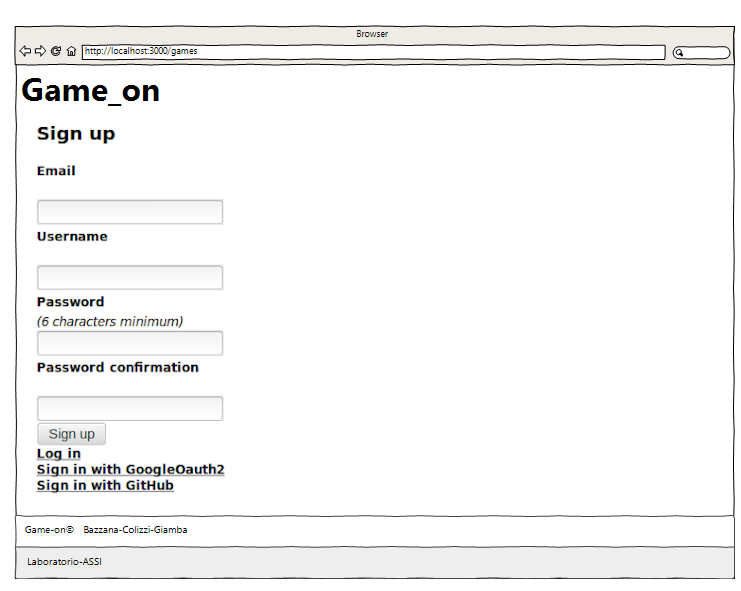
\includegraphics[width=0.45\textwidth]{mockup_registration}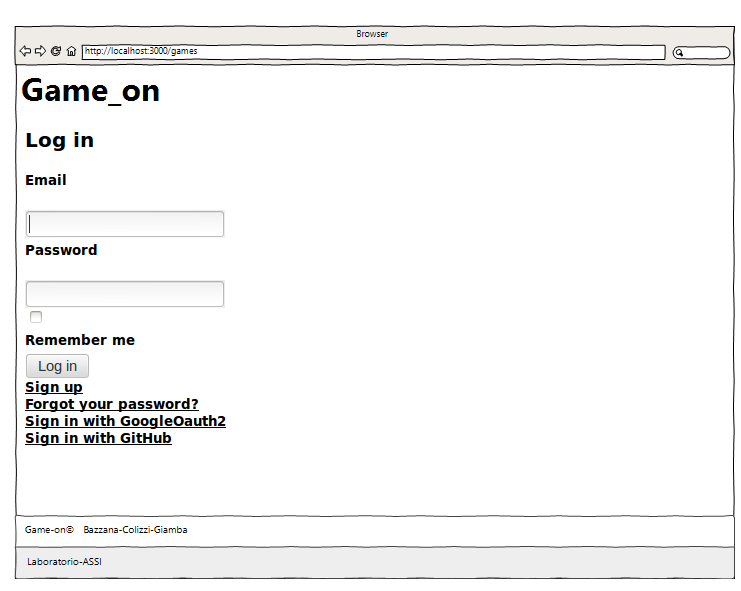
\includegraphics[width=0.45\textwidth]{mockup_login}
\caption{Mockup relativi alle user stories 1, 2 e 3}
\end{figure}

\subsection{Sezione giochi}

Ogni utente (anche un visitatore) può vedere l'elenco dei giochi presenti sulla piattaforma e effettuare ricerche all'interno di esso, mentre solo i giocatori possono giocare, caricare giochi e modificare o eliminare i propri. Per caricare un suo gioco sviluppato con \textit{Unity} un giocatore deve compilare il form presente in una pagina dedicata. Ogni giocatore può esprimere una preferenza su un gioco o fornire un voto positivo o negativo. Può inoltre vedere la lista dei suoi giochi preferiti.
\newline
Le user stories relative a queste funzionalità sono le seguenti:

\textit{
\begin{enumerate}
\item Come utente generico, voglio visualizzare l'elenco di tutti i giochi aggiunti nella piattaforma dagli altri giocatori.
\item Come utente generico,
voglio cercare un gioco specifico cercandolo per nome o per categoria, in modo che possa cercare solo ciò che mi interessa.
\item Come utente generico,
voglio ordinare i risultati di una ricerca, in modo che possa avere i risultati disposti secondo vari criteri.
\item Come giocatore, voglio inserire un gioco nella piattaforma, in modo che sia visibile agli altri utenti.
\item Come giocatore, voglio rimuovere un mio gioco dalla piattaforma, in modo che non sia più disponibile su di essa.
\item Come utente generico, voglio vedere le informazioni di un gioco.
\item Come giocatore, voglio giocare a un gioco.
\item Come giocatore proprietario di un gioco, voglio modificare la descrizione del gioco, così che lo possa mantenere aggiornato.
\item Come giocatore proprietario di un gioco, voglio rilasciare una patch del gioco, così da mostrare solo la versione più aggiornata.
\item Come giocatore, voglio assegnare o rimuovere un like o un dislike ad un gioco, in modo da fornire un feedback pubblico allo sviluppatore.
\item Come giocatore, voglio aggiungere/rimuovere un gioco ai miei preferiti, in modo che lo possa trovare nella mia lista preferiti.
\item Come giocatore, voglio visualizzare una pagina con tutti i miei giochi preferiti, in modo che siano tutti raggruppati in un unico posto.
\end{enumerate}
}

\begin{figure}[h!]
\centering
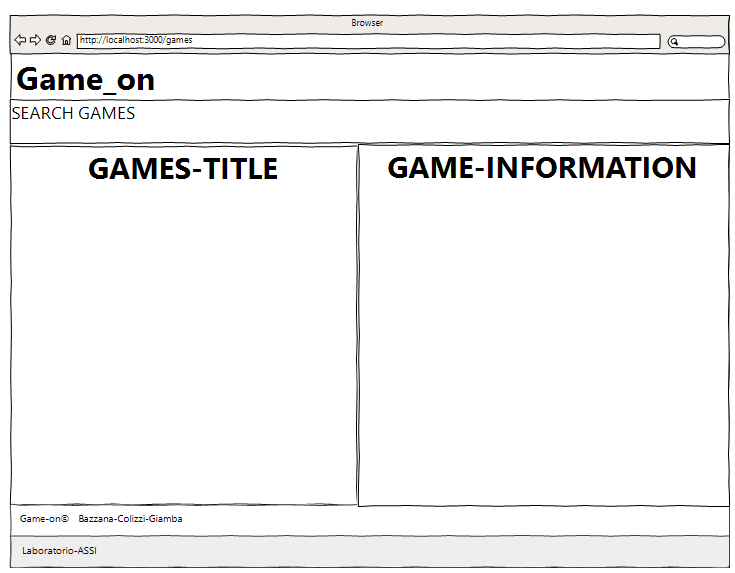
\includegraphics[width=0.45\textwidth]{mockup_games}
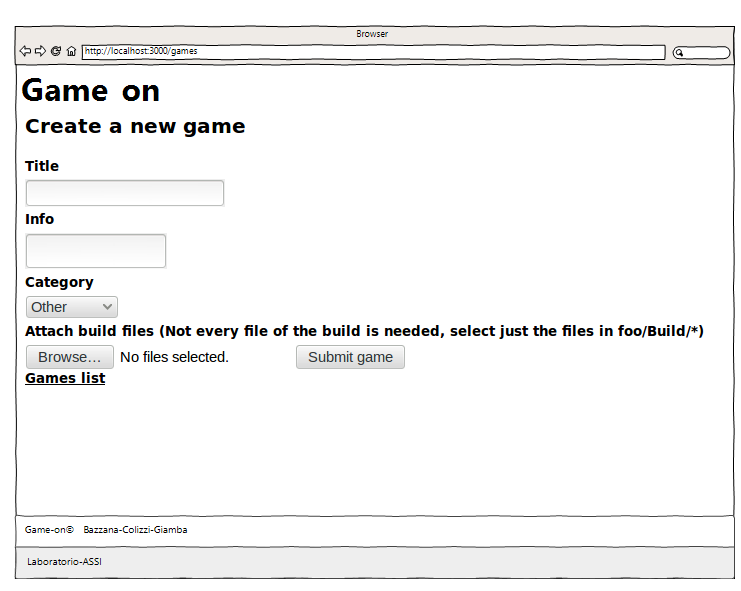
\includegraphics[width=0.45\textwidth]{mockup_add_game}
\caption{Mockup relativi alle user stories 1 e 4}
\end{figure}


\section{Metodologia utilizzata di conduzione del progetto ed organizzazione del lavoro}

Il gruppo di lavoro è formato da tre componenti: Davide Bazzana,
Giacomo Colizzi Coin e Renato Giamba.
\newline
\newline
Lo sviluppo del progetto è stato organizzato seguendo la metodologia
ASD (\textit{agile software development}).

Il calendario è stato suddiviso in iterazioni, in modo da definire
quante e quali user stories dovevano essere sviluppate in un certo
periodo di tempo. Subito dopo aver definito le user stories da
svluppare, esse sono state suddivise in gruppi, ciascuno affidato ad
una iterazione. Nella prima parte dello sviluppo, la durata di
ciascuna iterazione è stata di 3 settimane, successivamente però tale
durata è stata ridotta a 2 settimane, per accelerare lo sviluppo e
concludere il progetto rispettando la data di consegna che il gruppo
si era inizialmente proposto.  Ad ogni scadenza di una iterazione, ed
inizio di quella successiva, il gruppo si riuniva per discutere dei
traguardi raggiunti e di quelli da raggiungere in futuro. Lo scopo
principale di queste riunioni era infatti quello di assegnare a
ciascun componente del gruppo un insieme di user stories appartenti
alla successiva iterazione.  Questa scelta veniva fatta in base alla
propensione dei singoli componenti e alle competenze di ciascuno di
essi, sia acquisite in altre occasioni, sia acquisite durante lo
sviluppo del progetto stesso. Questo modus operandi ha fatto sì che i
vari componenti del gruppo, pur continuando a mantenere una visione
chiara del funzionamento complessivo dell'applicazione, si siano
specializzati in un suo ambito specifico.

\subsection{Servizi di terze parti utilizzati}

Per gestire ed analizzare l'andamento dello sviluppo del progetto è
stato utilizzato il tool \textit{PivotalTracker}.

Questo tool ha permesso al gruppo di tenere traccia di tutte le user
stories e delle loro relative informazioni: il contenuto della user
story, il suo stato di sviluppo (unstarted, started, finished, delivered,
rejected, accepted), l'iterazione alla quale faceva riferimento, il
componente responsabile del suo sviluppo, il livello di difficoltà, ed
altro. Per tutta la durata del progetto, ciascun componente aveva la
possibilità di consultare e modificare tali informazioni.

Infine, \textit{PivotalTracker}, ha reso possibile valutare in tempo
reale le informazioni relative all'andamento dello sviluppo, come la
sua velocità e volatilità.
\newline
\newline
Per il controllo di versione è stato scelto il software \textit{Git},
mentre, come servizio di hosting per la repository del progetto, è
stato scelto \textit{GitHub}.

La metodologia impiegata dal gruppo per l'utilizzo dei branch della
repository è stata quella di creare un branch per ciascuna user story
in sviluppo e di mantenere un branch chiamato ``\textit{master}'' come
branch di mantenimento di una versione stabile.

La procedura di controllo del nuovo software prodotto invece, è stata
quella di \textit{peer review}. Infatti, ogni volta che un componente
del gruppo completava l'implementazione di una user story, sottoponeva
il suo lavoro al giudizio degli altri. Questa procedura veniva svolta
facendo uso del meccanismo di pull request offerto da
\textit{GitHub}. Se il resto dei componenti del gruppo riteneva il
lavoro svolto adeguato, la \textit{pull request} veniva accettata e si
procedeva col \textit{merging} del branch in questione con il branch
``\textit{master}'', altrimenti, il componente, o i componenti, che
non ritenevano il lavoro svolto sufficiente, commentavano la
\textit{pull request} evidenziando eventuali errori da correggere o
miglioramenti da apportare.
\newline
\newline
Infine è stata sfruttata la possibilità di integrare un progetto su
\textit{PivotalTracker} con una repository su \textit{GitHub}.

Con questa funzionalità abilitata, tutti gli avanzamenti di un branch
relativo ad una user story venivano comunicati da \textit{GitHub} a
\textit{PivotalTracker}, provocando così l'aggiornamento automatico
dello stato della user story su \textit{PivotalTracker}.

\subsection{Statistiche di sviluppo}

Il progetto è iniziato il 21 marzo 2020 e finito il 16 settembre
2020, con una durata totale di 25 settimane e 5 giorni.
\newline
\newline
La tabella seguente mostra alcune statistiche sul contributo di
ciascun componente del gruppo. Pur riportando il numero esatto di
commit, file e righe prodotte da ciascuno, i seguenti dati sono
indicativi. Infatti, ad esempio, una percentuale non indifferente del
numero di file e linee indicate, non costituisce un contributo diretto
del componente, bensì deriva dalle gemme e dai file di terze parti
utilizzati, come quelli prodotti da \textit{Unity 3D} per il
gioco di test ``\textit{Kloby}''.

\vspace{1cm}
\begin{tabular}{l|r|r|r}
  \textbf{Developer} & \textbf{Commits} & \textbf{Files changed} & \textbf{Total lines} \\
  \hline
  Davide Bazzana & 111 & 366 & 7428 \\
  \hline
  Giacomo Colizzi Coin & 88 & 506 & 2680 \\
  \hline
  Renato Giamba & 42 & 183 & 1110 \\
  \hline
\end{tabular}


\backmatter
\cleardoublepage
\phantomsection
\addcontentsline{toc}{chapter}{\bibname}
	
\end{document}
